\appendix
\chapter{Appendix}

\pagebreak

\begin{minipage}{\linewidth}
    \lstinputlisting[language=Kotlin,caption=Algorithmus zum Name-Matching,label=lst:name_matching]{../images/StringMatching.kt}
\end{minipage}

\pagebreak

\begin{figure}[h]
    \centering
    \begin{subfigure}{0.8\textwidth}
        \centering
        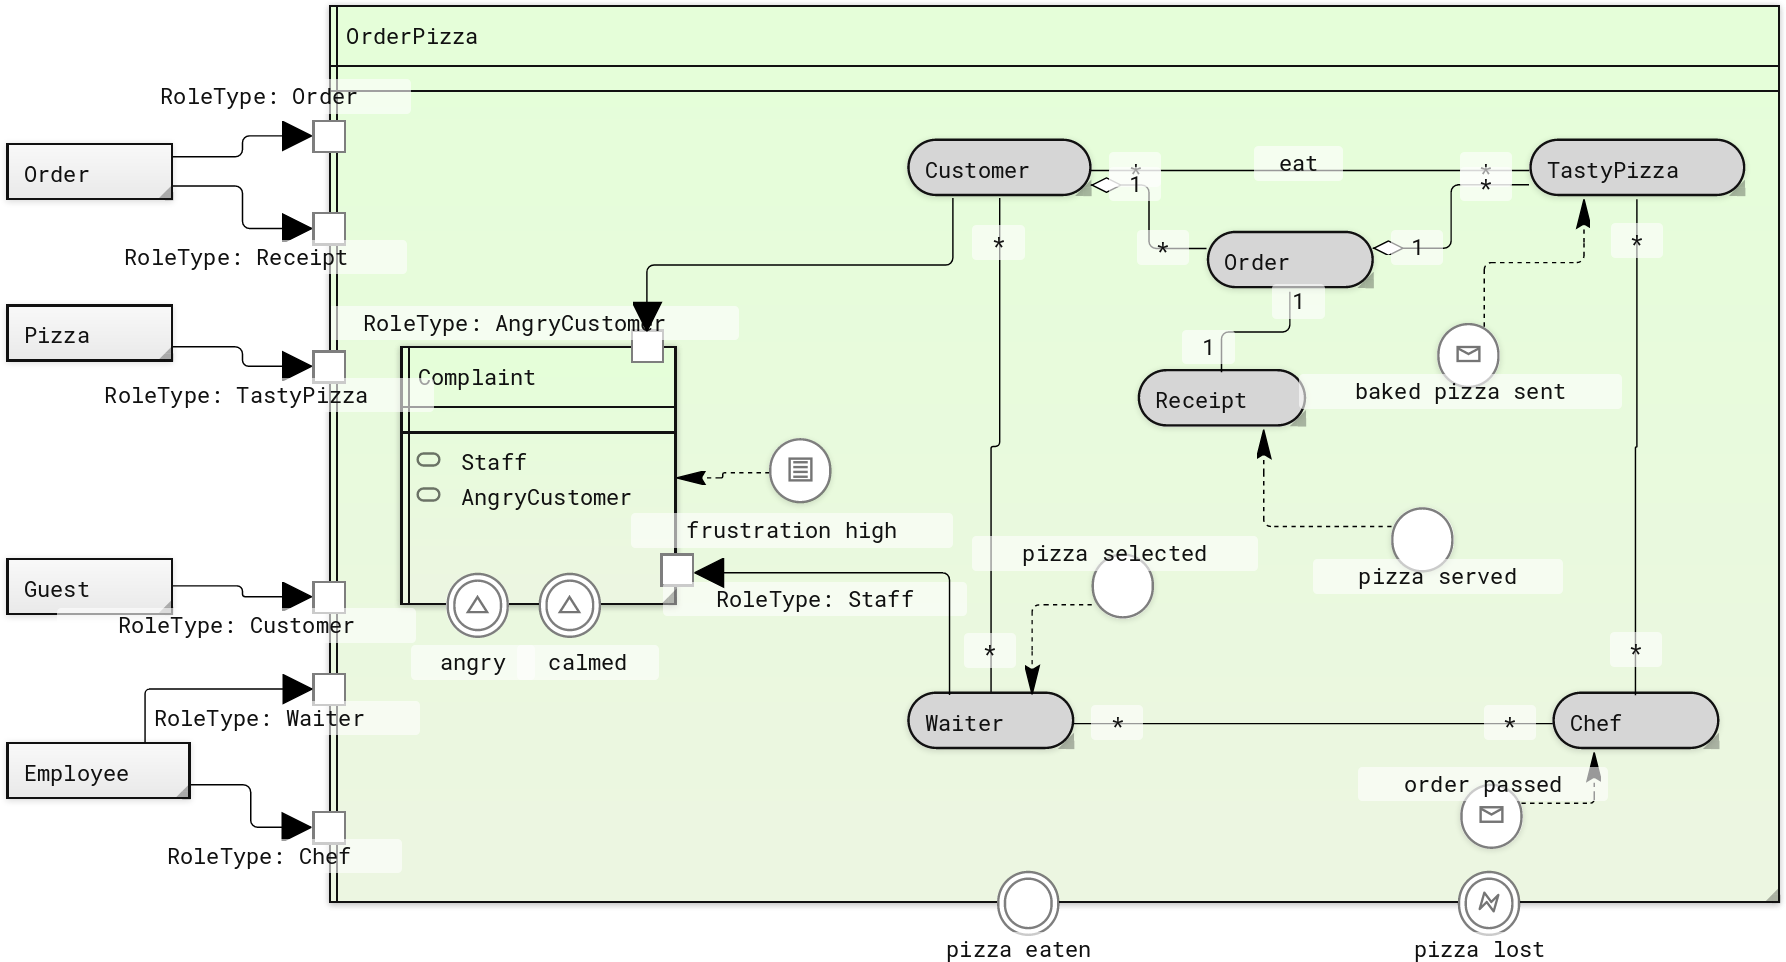
\includegraphics[width=\textwidth,keepaspectratio]{../images/example/bros-rule3.png}%
        \caption{Entwurf 2 für das BROS-Modell der Pizzabestellung}%
        \label{fig:pizzaBros3}
    \end{subfigure}
    \begin{subfigure}{0.8\textwidth}
        \centering
        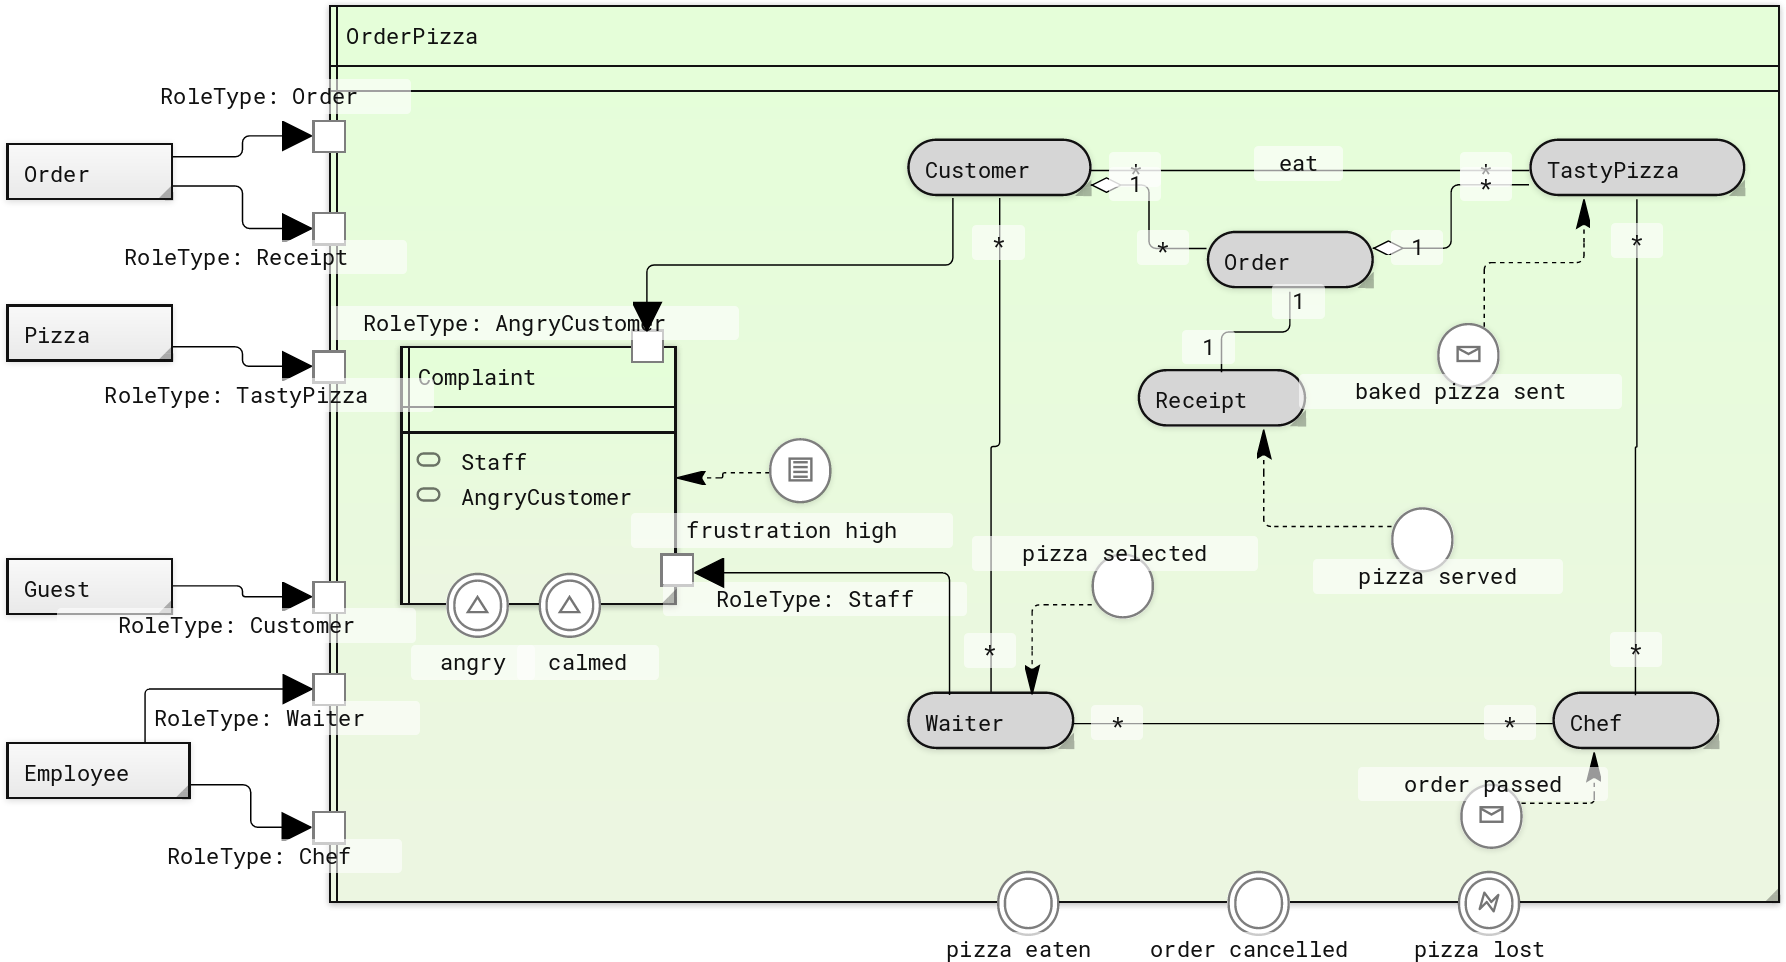
\includegraphics[width=\textwidth,keepaspectratio]{../images/example/bros-rule4.png}%
        \caption{Entwurf 3 für das BROS-Modell der Pizzabestellung}%
        \label{fig:pizzaBros4}
    \end{subfigure}
    \begin{subfigure}{0.8\textwidth}
        \centering
        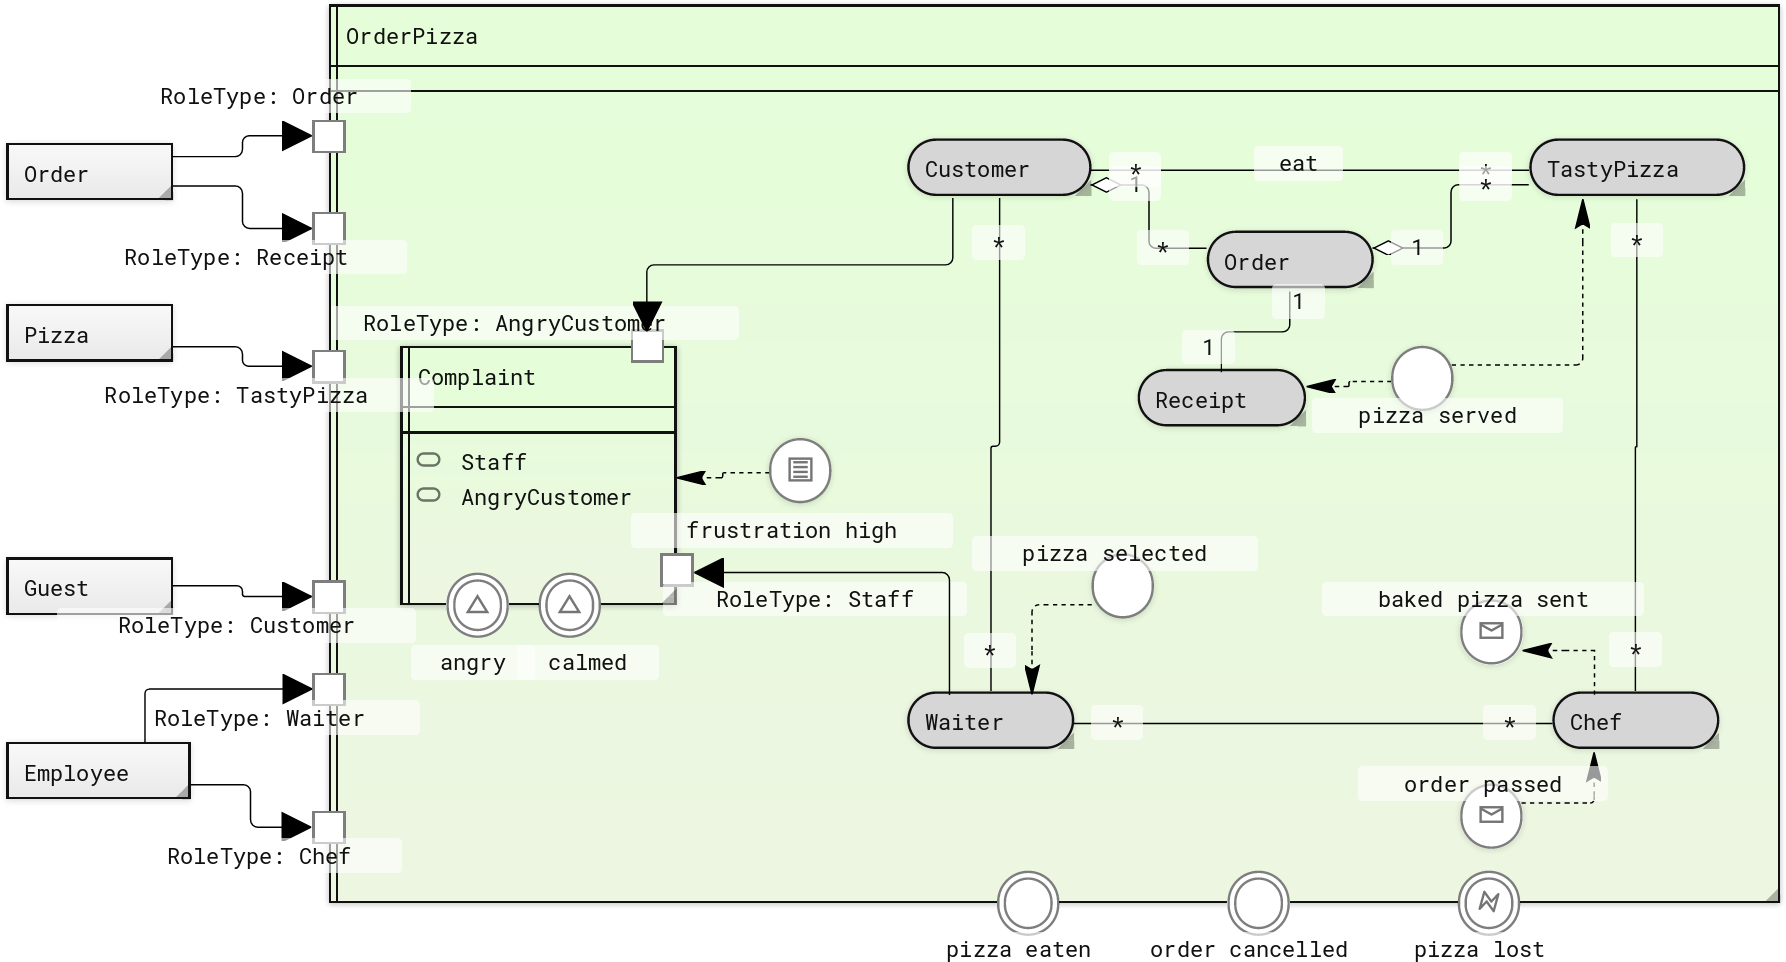
\includegraphics[width=\textwidth,keepaspectratio]{../images/example/bros-rule5.png}%
        \caption{Entwurf 4 für das BROS-Modell der Pizzabestellung}%
        \label{fig:pizzaBros5}
    \end{subfigure}
    \caption{Entwurfsschritte für das BROS-Modell der Pizzabestellung}%
    \label{fig:pizzaBrosSteps}
\end{figure}

\pagebreak

\begin{minipage}{\linewidth}
    \lstinputlisting[language=Kotlin,caption=Implementierung der Datei Rule6BrosEvent.kt,label=lst:Rule6BrosEvent]{../images/Rule6BrosEvent.kt}
\end{minipage}
